\documentclass{beamer}

%\setbeamertemplate{theorems}[numbered]
\usepackage{iipr_beamer}
\usetheme{Madrid}

\makeatletter
\setbeamertemplate{footline}
{
  \leavevmode%
  \hbox{%
  \begin{beamercolorbox}[wd=.4\paperwidth,ht=2.25ex,dp=1ex,center]{author in head/foot}%
    \usebeamerfont{author in head/foot}\insertsection
  \end{beamercolorbox}%
  \begin{beamercolorbox}[wd=.35\paperwidth,ht=2.25ex,dp=1ex,center]{title in head/foot}%
    \usebeamerfont{title in head/foot}\insertsubsection
  \end{beamercolorbox}%
  \begin{beamercolorbox}[wd=.25\paperwidth,ht=2.25ex,dp=1ex,right]{date in head/foot}%
    \usebeamerfont{date in head/foot}\insertshortdate{}\hspace*{1em}
    \insertframenumber{} / \inserttotalframenumber\hspace*{3ex} 
  \end{beamercolorbox}}%
  \vskip0pt%
}
\makeatother

\title{\large{\textsc{Complexity Analysis of Polynomial Algorithms}}}
\subtitle{\textsc{Final Degree Project}}
\author{\vspace{-0.4cm}\\
Ignacio Iker Prado Rujas}
\institute{
	\vspace{-0.3cm} \\
	\protect
\includegraphics[scale=0.75]{ucm.eps}\\
	\vspace{0.2cm}
	Complutense University of Madrid (UCM) \\
	Double Degree in Mathematics and Computer Science\\
	\vspace{0.3cm}
	Tutors: \\
	Juan R. Delgado, Jos\'e F. Fernando \textit{\&} Jos\'e M. Gamboa \\
	\vspace{0.1cm}
	Department of Algebra, Faculty of Mathematics\\
	\vspace{-0.3cm}
}
\date{July 13\textsuperscript{th}, 2016}

\setbeamertemplate{blocks}[rounded][shadow=true]
\setbeamertemplate{background canvas}[vertical shading][bottom=white,top=structure.fg!25]
\setbeamertemplate{sidebar canvas left}[horizontal shading][left=white!40!black,right=black]
\beamertemplatenavigationsymbolsempty %Supress navigation bar

\newcommand{\beginbackup}{
   \newcounter{framenumbervorappendix}
   \setcounter{framenumbervorappendix}{\value{framenumber}}
}
\newcommand{\backupend}{
   \addtocounter{framenumbervorappendix}{-\value{framenumber}}
   \addtocounter{framenumber}{\value{framenumbervorappendix}} 
}


%\usefonttheme{professionalfonts} % using non standard fonts for beamer
\usefonttheme{serif}

\setbeamercolor{block title}{bg=black!10!blue!90} % Color of the block
\setbeamertemplate{section in toc shaded}[default][70] %Shaded table of contents

\begin{document}

\frame{\titlepage}

\section{Introduction to polynomial images of $R^n$}
\begin{frame}
\frametitle{Table of contents}
\tableofcontents[currentsection]
\end{frame} 

\subsection{The problem}
\begin{frame}
\frametitle{Introduction to polynomial images of $R^n$}
$\cdot$ Let $R$ be a real closed field.\vspace{0.3cm}

\begin{block}{Theorem (Tarski-Seidenberg, 1951)}
The image of every polynomial map $f:R^m\to R^n$ is a \hyperref[semialgSet]{semialgebraic subset} of $R^n$.
\end{block}
 
\vspace{1cm}

\begin{block}{`Inverse problem' (Proposed by J.M. Gamboa, 1990)}
Characterize the semialgebraic subsets of $R^n$ that are polynomial images of some $R^m$.
\end{block}

\end{frame}

\subsection{Examples}
\begin{frame}
\frametitle{Some introductory examples}
%\vspace{-1cm}
\begin{enumerate}[(i)]
\item $[0,+\infty)$ is the image of $\R$ under $f:\R\to\R, x\mapsto x^2$.  
\vspace{0.3cm}

\item $(0,+\infty)$ \textbf{is not} the image of any polynomial map $\R\to\R$.   
\vspace{0.3cm}

\item $(0,+\infty)$ is the image of $f:\R^2\to\R,\, (x,y)\mapsto (xy-1)^2+y^2.$    
\vspace{0.3cm}

\item $S:=\set{x^2+y^2>1}\subset R^2$ \textbf{is not} a polynomial image of $R^2$.  
\vspace{0.3cm}

\item $\H:=\set{y>0}\subset\R^2$ is the image of the polynomial map $$\R^2\to\R^2,\, (x,y)\mapsto \big(y(xy-1),(xy-1)^2+x^2\big).$$  
\vspace{-0.4cm}

\item $S_1:=\set{xy<1}\subset R^2$ and $S_2:=\set{xy>1,x>0}\subset R^2$ \textbf{are not} polynomial images of $R^2$.  
\vspace{0.3cm}

\item $S_3:=R^2\setminus\set{(0,0)}$ is the image of the polynomial map $$\R^2\to\R^2,\, (x,y)\mapsto \big(xy-1,(xy-1)x^2-y\big).$$
%\vspace{0.2cm}

\end{enumerate}
\end{frame}

\subsection{Main results}
\begin{frame}
\frametitle{Statement of the main results}

\begin{block}{Theorem 1.9}
Let $n\ge2$. For every finite set $F\subset R^n$, the semialgebraic set $R^n\setminus F$ is a polynomial image of $R^n$.
\end{block} 
\vspace{0.4cm}

\begin{block}{Theorem 1.10}
Let $n\ge 2$. Given independent linear forms $h_1,\dots,h_r$ of $R^n$, the open semialgebraic set $\set{h_1>0,\dots,h_r>0}$ is a polynomial image of $R^n$.
\end{block} 
\vspace{0.4cm}

\begin{block}{Theorem 1.11}
The open quadrant $\Qu:=\{x>0,y>0\}$ is a polynomial image of $R^2$.
\end{block}
\end{frame}

\section{The open quadrant $\Qu$ problem}
\begin{frame}
\frametitle{Table of contents}
\tableofcontents[currentsection]
\end{frame} 

\subsection{The first proof: $g:=\P\circ Q\circ H$}
\begin{frame}
\frametitle{The first proof: $g:=\P\circ Q\circ H$} 
$\star$ The map $H:\R^2\to\R^2$ transforms $\R^2$ in $\R^2\setminus \set{(0,0),(-1,0)}$:
$$
H(\x,\y) := \big(\x\y+1,\ \x^2(\x\y+1)(\x\y+2)+\y\big).
$$	
 

$\star$ The map $Q:\R^2\to\R^2$ maps $(0,0) \mapsto (0,-1)$ and $(-1,0) \mapsto (-1,0)$: 
$$
Q(\x,\y)= (\x,\y-\x-1).
$$
 

$\star$ The map $\P := (\F, \G)$ transforms $\R^2$ into $\Qu \sqcup \set{(1,0),(0,1)}$ and $\P^{-1}\big(\set{(1,0),(0,1)}\big) = \set{(0,-1),(-1,0)}$:
\begin{equation*}\label{eq:firstMap}
\boxed{
\begin{aligned}
\F({\tt x},{\tt y})&:=(1-{\tt x}^3{\tt y}+{\tt y}-{\tt x}{\tt y}^2)^2+({\tt x}^2{\tt y})^2, \\
\G({\tt x},{\tt y})&:=(1-{\tt x}{\tt y}+{\tt x}-{\tt x}^4{\tt y})^2+({\tt x}^2{\tt y})^2. \\
\end{aligned}
}
\end{equation*}
 

$\star$ Then $g\big(\R^2\big) = \Qu$, where:
$$
g:=\P\circ Q\circ H:\R^2\longrightarrow\R^2.
$$
\end{frame}

\subsection{The short proof: $f:=\HH\circ\GG\circ\FF$}
\begin{frame}
\frametitle{The short proof: $f:=\HH\circ\GG\circ\FF$} 
$\star$ The map $f:=\HH\circ\GG\circ\FF:\R^2\to\R^2$ verifies $f\big(\R^2\big) = \Qu$, where:
\begin{equation*}\label{eq:secondMap}
\boxed{
\begin{aligned}
\FF:\R^2\to\R^2,\ (x,y)&\mapsto\big((xy-1)^2+x^2,\ (xy-1)^2+y^2\big),\\
\GG:\R^2\to\R^2,\ (x,y)&\mapsto\big(x,\ y(xy-2)^2+x(xy-1)^2\big),\\
\HH:\R^2\to\R^2,\ (x,y)&\mapsto\big(x(xy-2)^2+\tfrac{1}{2}xy^2,\ y\big). \\
\end{aligned}
}
\end{equation*}
\vspace{-0.4cm}

\begin{columns}
\begin{column}{0.5\textwidth}
\begin{figure}
\begin{tikzpicture}
\node[anchor=south west,inner sep=0] (img)at (0,0) {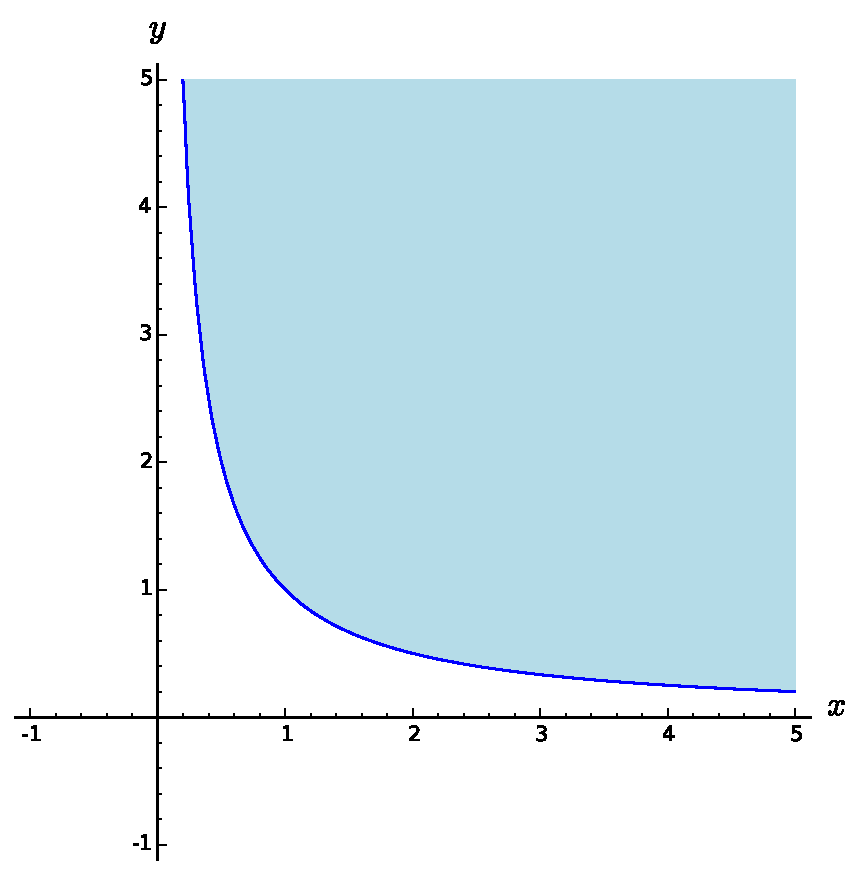
\includegraphics[width=0.837\textwidth]{plots/ch2_07_A.pdf}};
\path ($(img.north west)!0.6!(img.north east)$)|-coordinate(c1)($(img.south east)!0.7!(img.north east)$);% c1: lugar donde poner \mathscr{A}
\draw (c1) node {\large{$\mathscr{A}$}};
\end{tikzpicture}
%\caption{$\mathscr{A}:=\set{xy\ge 1}\ \cap\, \Qu$.}
\end{figure}
\end{column}

\begin{column}{0.5\textwidth}
\begin{center}
\resizebox{5cm}{5cm}{%
\begin{tikzpicture}
\node[anchor=south west,inner sep=0] (img)at (0,0) {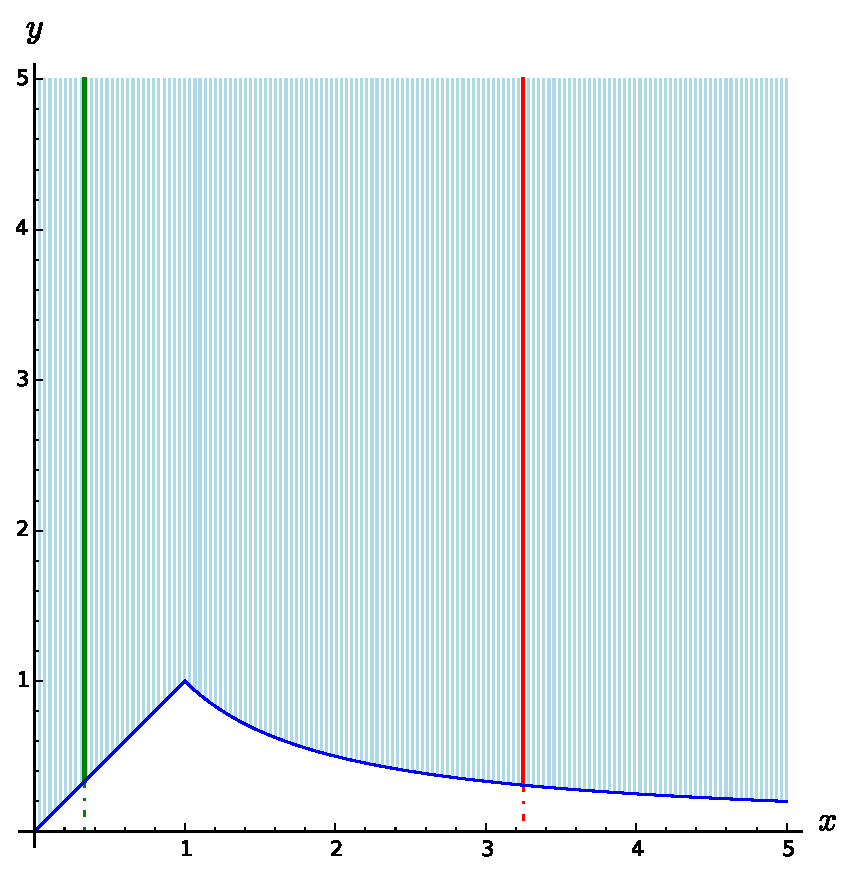
\includegraphics[width=1\textwidth]{plots/ch2_09_B_vert.pdf}};
\path ($(img.north west)!0.8!(img.north east)$)|-coordinate(c1)($(img.south east)!0.8!(img.north east)$); % Para \mathscr{B}
\path ($(img.north west)!0.1!(img.north east)$)|-coordinate(c2)($(img.south east)!0.89!(img.north east)$); % Para la flecha de x_0
\path ($(img.north west)!0.613!(img.north east)$)|-coordinate(c3)($(img.south east)!0.89!(img.north east)$); % Para la flecha de x_1
\path ($(img.north west)!0.1!(img.north east)$)|-coordinate(c4)($(img.south east)!0.105!(img.north east)$); % Para [
\path ($(img.north west)!0.613!(img.north east)$)|-coordinate(c5)($(img.south east)!0.101!(img.north east)$); % Para [
\path ($(img.north west)!0.1!(img.north east)$)|-coordinate(c6)($(img.south east)!0.01!(img.north east)$); % Para x_0
\path ($(img.north west)!0.613!(img.north east)$)|-coordinate(c7)($(img.south east)!0.01!(img.north east)$); % Para x_1
\path ($(img.north west)!0.28!(img.north east)$)|-coordinate(c8)($(img.south east)!0.55!(img.north east)$); % Para B_{x_0}
\path ($(img.north west)!0.79!(img.north east)$)|-coordinate(c9)($(img.south east)!0.35!(img.north east)$); % Para B_{x_1}
\draw (c1) node {\Large{$\mathscr{B}$}};
\draw (c2) node {\large{\color[rgb]{0,0.392157,0}{$\uparrow$}}};
\draw (c3) node {\large{\color[rgb]{1,0,0}{$\uparrow$}}};
\draw (c4) node {\large{\color[rgb]{0,0.392157,0}{\rotatebox[origin=c]{90}{[}}}};
\draw (c5) node {\large{\color[rgb]{1,0,0}{\rotatebox[origin=c]{90}{[}}}};
\draw (c6) node {\large{\color[rgb]{0,0.392157,0}{$x_0$}}};
\draw (c7) node {\large{\color[rgb]{1,0,0}{$x_1$}}};
\draw (c8) node {\large{\color[rgb]{0,0.392157,0}{$\set{x_0} \times \mathscr{B}_{x_0}$}}};
\draw (c9) node {\large{\color[rgb]{1,0,0}{$\set{x_1} \times \mathscr{B}_{x_1}$}}};
\end{tikzpicture}
}
\end{center}
\end{column}
\end{columns}

\end{frame}

\begin{frame}
\frametitle{The short proof}
\begin{block}{Lemma 3.1}
The polynomial map $\FF$ verifies that $\mathscr{A}\subset\FF(\R^2)\subset\Qu$.
\end{block}
\begin{block}{Lemma 3.2}
The polynomial map $\GG$ verifies that $\mathscr{B}\subset\GG(\mathscr{A})\subset\GG(\Qu)\subset\Qu$.
\end{block}
\begin{block}{Lemma 3.3}
The polynomial map $\HH$ verifies that $\HH(\mathscr{B})=\HH(\Qu)=\Qu$.
\end{block}

$$
\!\!\!\Qu\overset{3.3}{=}\HH(\mathscr{B})\!\overset{3.2}{\subset}\!(\HH\circ\GG)(\mathscr{A})
\!\overset{3.1}{\subset}\!(\HH\circ\GG\circ\FF)(\R^2) \!\overset{3.1}{\subset}\!(\HH\circ\GG)(\Qu) \!\overset{3.2}{\subset}\!\HH(\Qu)\overset{3.3}{=}\Qu.
$$
\end{frame}

\subsection{The topological proof: $\FFF=f_2\circ f_1$}
\begin{frame}
\frametitle{The topological proof: $\FFF=f_2\circ f_1$} 
$\star$ The map $f_1(\x,\y):=\big(\x^2,\,\y^2\big)$ verifies $f_1\big(\R^2\big)=\overline{\Qu}:=\set{x\ge 0,y\ge 0}$.
\vspace{0.5cm}

$\star$ The map $f_2:=h\circ g$, where $g:\overline{\Qu}\to\R^3,\ h:\R^3\to\R^2$ and:% \vspace{-0.2cm}
\begin{align*}
g(\x,\y)&:=\big(\x\y^2+\x^2\y-\y-1,\,\x^{3/2}\y,\,\x^3\y+\x\y-\x-1\big),\\
h(\x,\y,\z)&:=\big(\x^2+\y^2,\,\y^2+\z^2\big),
\end{align*}%\vspace{-0.5cm} 
verifies that $f_2(\overline{\Qu}) = \Qu$.
\vspace{0.5cm}

$\star$ The map $\FFF:= (\FFF_1, \FFF_2):\R^2\to\R^2$ defined as:
\begin{equation*}\label{eq:thirdMap}
\boxed{
\begin{aligned}
\FFF_1({\tt x}, {\tt y}) := ({\tt x}^2{\tt y}^4+{\tt x}^4{\tt y}^2-{\tt y}^2-1)^2+{\tt x}^6{\tt y}^4,\\
\FFF_2(\x, \y) := ({\tt x}^6{\tt y}^2+{\tt x}^2{\tt y}^2-{\tt x}^2-1)^2+{\tt x}^6{\tt y}^4.
\end{aligned}
}
\end{equation*}
Note that $\FFF = f_2 \circ f_1$, so we have that $\FFF\big(\R^2\big) = \Qu$.
\end{frame}

\begin{frame}
\frametitle{The topological proof: The key step}

\begin{columns}
\begin{column}{0.5\textwidth}
\begin{center}The boundary map $\partial\tilde{\phi}_M:\partial\tilde{\overline{\Rr}}_M\rightarrow\R^3$ meets transversally once $\D_1$.
\end{center}\begin{figure}[!ht]
\begin{center}
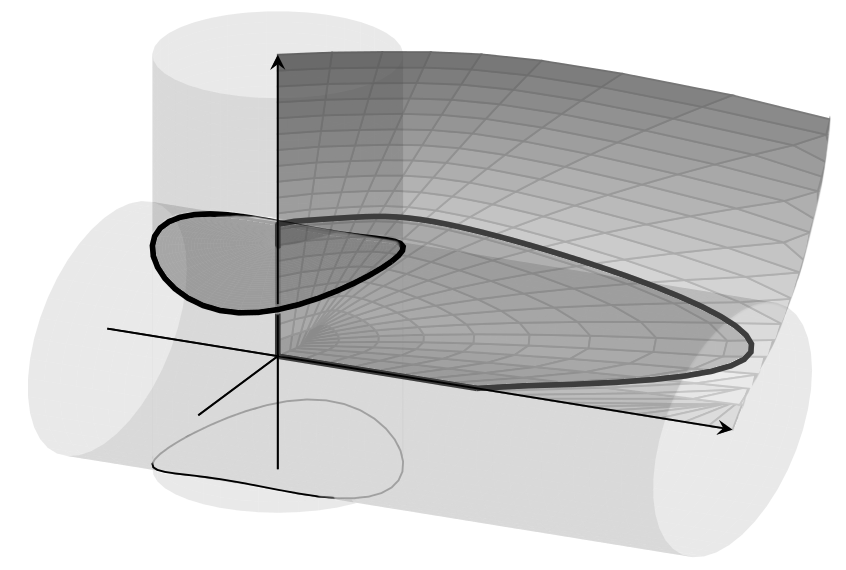
\includegraphics[height=4cm]{plots/ch3_02_B2.png}
\end{center}
\end{figure}
\end{column}
\begin{column}{0.5\textwidth}
\begin{center}The boundary map $\partial\tilde{\phi}_M:\partial\tilde{\overline{\Rr}}_M\rightarrow\R^3$ meets transversally once $\D_2$.
\end{center}\begin{figure}[!ht]
\begin{center}
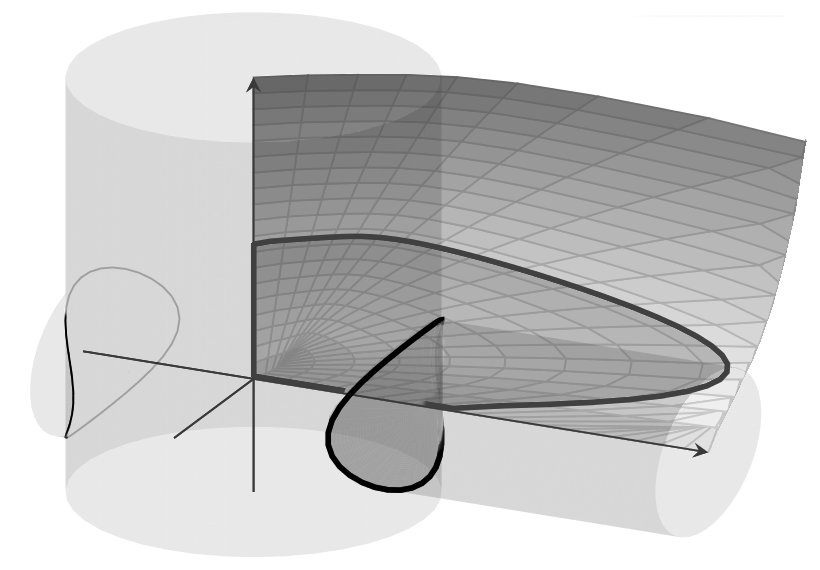
\includegraphics[height=4cm]{plots/ch3_01_A2.png}
\end{center}
\end{figure}
\end{column}
\end{columns}

\end{frame}

\section{Complexity analysis}
\begin{frame}
\frametitle{Table of contents}
\tableofcontents[currentsection]
\end{frame} 

\subsection{Some new candidates}
\begin{frame}
\frametitle{Some new candidates}
$\star$ Polynomial maps $\R^2\to\R^2$ whose images ``should be" $\Qu$:

\begin{align*}
\cdot\ \mathcal{N}_1(x,y):=\big(&x^4y^4+(x^2y+xy^2-1)^2(y^2+1),\\
&x^4y^4+(x^2y+xy^2-1)^2(x^2+1)\big).
\end{align*}

\begin{align*}
\cdot\ \mathcal{N}_2(x,y):=\big(&x^2y^2+(x^2y+xy^2-1)^2(y^2+1),\\
&x^2y^2+(x^2y+xy^2-1)^2(x^2+1)\big).
\end{align*}

\begin{align*}
\cdot\ \mathcal{N}_3(x,y):=\big(&x^6y^4+(x^2y+xy^2-1)^2(y^2+1),\\
&x^4y^6+(x^2y+xy^2-1)^2(x^2+1)\big).
\end{align*}

\end{frame}


\subsection{Measurements of the complexity}
\begin{frame}
\frametitle{Measurements of the complexity}

$\star$ \textbf{Optimal algebraic structure:} Minimum total degree and sparseness (minimum number of monomials).
\vspace{0.4cm} 

$\star$ \textbf{Optimal multiplicative complexity:} Minimum number of non-scalar products.
\vspace{0.4cm}

\begin{table}[t]
\begin{center}
\begin{tabular}{c || c | c | c}
& Total degree & \begin{tabular}[c]{@{}c@{}}Total number\\of monomials\end{tabular} & \begin{tabular}[c]{@{}c@{}}Non-escalar\\complexity\end{tabular}\\ \hline \hline
$g = \P\circ Q \circ H$ & 56 & 167 & 13 \\ \hline
$f=\HH\circ\GG\circ\FF$ & 72 &  350 & 11\\ \hline
$\FFF = f_2 \circ f_1$ & 28 & 22 & 11\\ \hline	
$\mathcal{N}_1$&16&24&10 \\ \hline
$\mathcal{N}_2$&16&26&8 \\ \hline
$\mathcal{N}_3$&20&26&13 \\	
\end{tabular}
\end{center}
\end{table}
\end{frame}

\subsection{Computational analysis}
\begin{frame}
\frametitle{Uniformly distributed points contained in a square}
\begin{table}[ht!]
\begin{center}
\begin{tabular}{c || c | c | c}
& $g = \P\circ Q\circ H$ & $f=\HH\circ\GG\circ\FF$ & $\FFF$ \\ \hline \hline
$\PP_1\! \leadsto\! [-10, 10]^2$ & 0.19 s & 0.17 s & 0.07 s \\ \hline
$\PP_2\! \leadsto\! [-100, 100]^2$ & 17.38 s & 16.23 s & 6.88 s \\ \hline
$\PP_3\! \leadsto\! [0, 1]^2$ & 410.73 s & 389.74 s & 155.09 s \\ \hline
$\PP_4\! \leadsto\! [-1, 1]^2$ & 408.88 s & 392.34 s & 155.29 s \\ \hline
$\PP_5\! \leadsto\! [-10, 10]^2$ & 17.10 s & 15.45 s & 7.00 s \\ \hline
$\PP_6\! \leadsto\! [-10, 10]^2$ & 1633.50 s & 1640.01 s & 625.11 s \\
\end{tabular}
\end{center}
\end{table}

\begin{figure}
\vspace{-0.25cm}
\begin{subfigure}{.32\linewidth}\centering
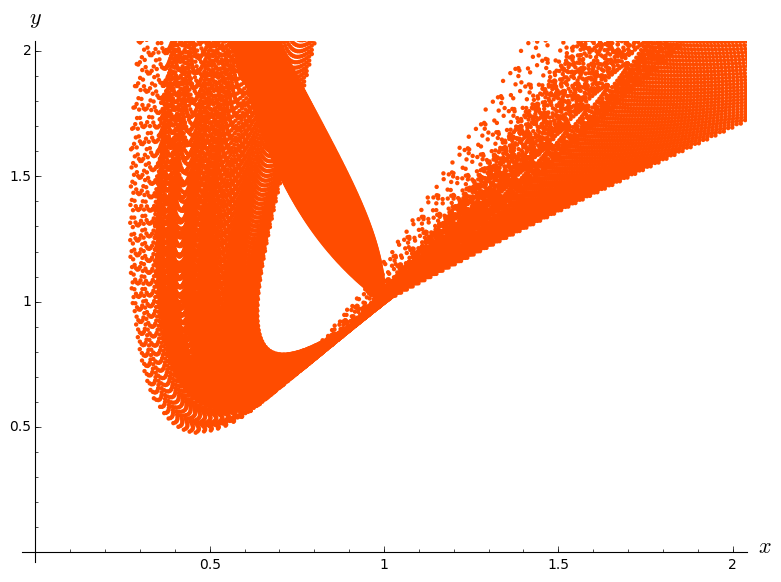
\includegraphics[width=1\textwidth]{plots/ch5_08_P4prime.png}
\caption{$g(\PP_4)$.}
\end{subfigure}
\begin{subfigure}{.32\linewidth}\centering
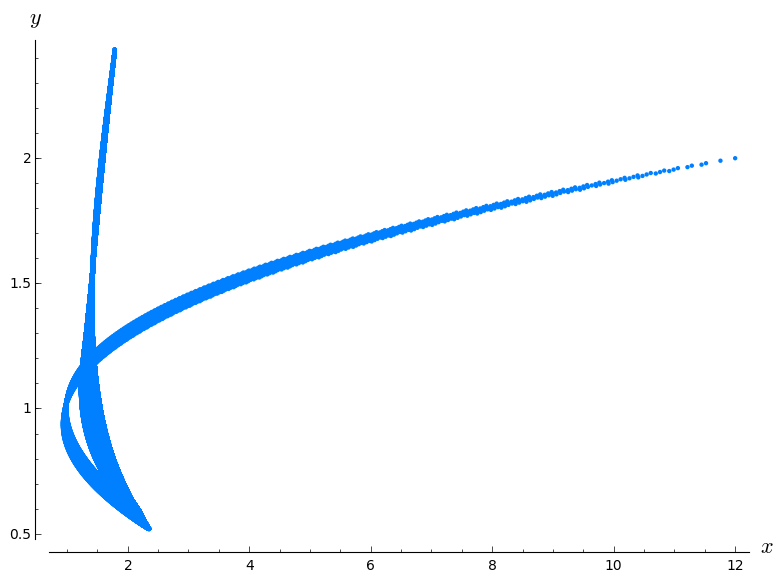
\includegraphics[width=1\textwidth]{plots/ch5_05_P3.png}
\caption{$f(\PP_3)$.}
\end{subfigure}
\begin{subfigure}{.32\linewidth}\centering
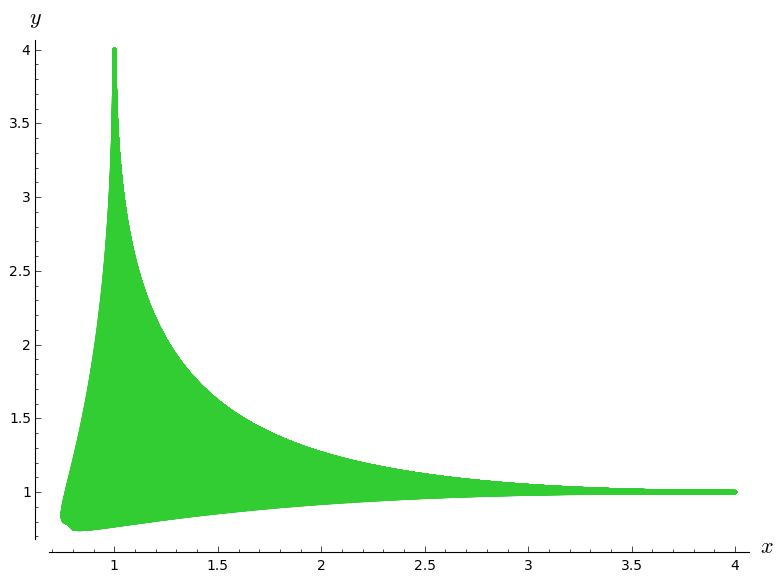
\includegraphics[width=1\textwidth]{plots/ch5_06_P3.png}
\caption{$\FFF(\PP_3)$.}
\end{subfigure}

\end{figure}

\end{frame}

\begin{frame}
\frametitle{Uniformly distributed points in $[-10, 10] \times [-10, 10]$}

\begin{figure}
\vspace{-0.2cm}
\begin{subfigure}{.38\linewidth}\centering
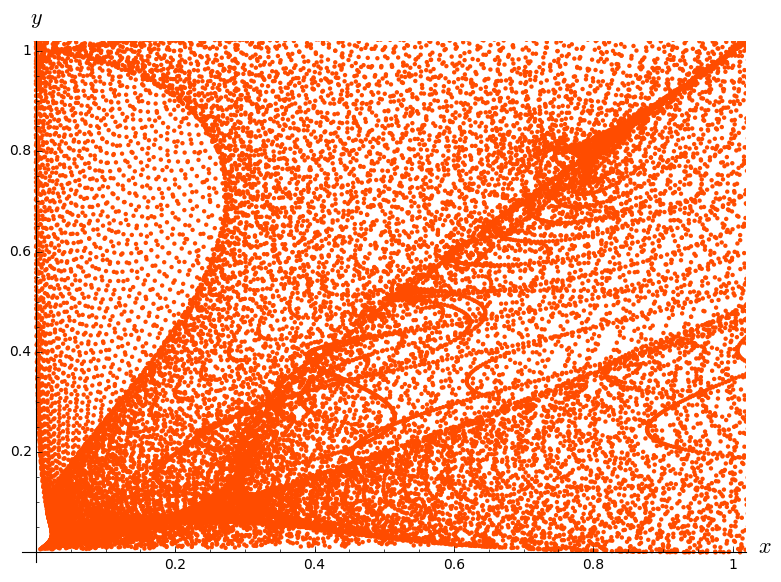
\includegraphics[width=1\textwidth]{plots/ch5_17_P6prime.png}
\vspace{-0.1cm}\caption{$g(\PP_6)\leadsto 1633.50$ s.}
\end{subfigure}
\hspace{0.8cm}
\begin{subfigure}{.38\linewidth}\centering
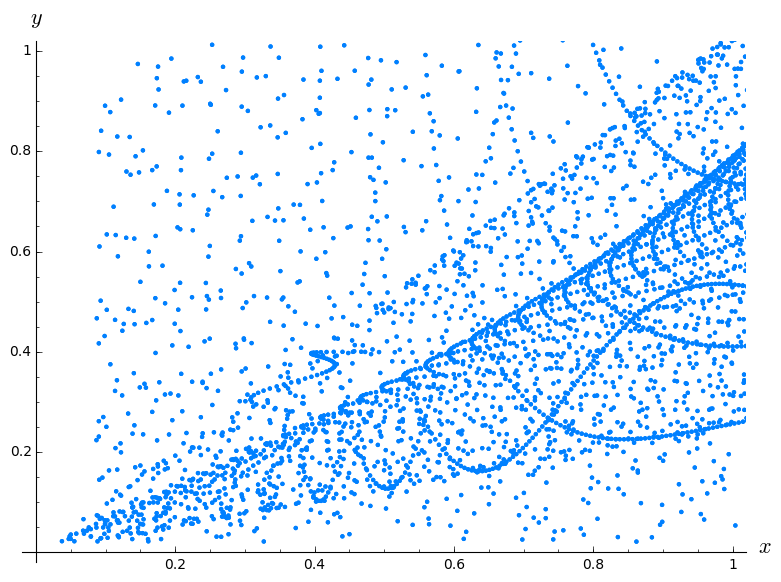
\includegraphics[width=1\textwidth]{plots/ch5_20_P6prime.png}
\vspace{-0.1cm}\caption{$g(\PP_6)\leadsto 1640.01$ s.}
\end{subfigure}\\[1ex]

%\vspace{-0.1cm}
\begin{subfigure}{.38\linewidth}\centering
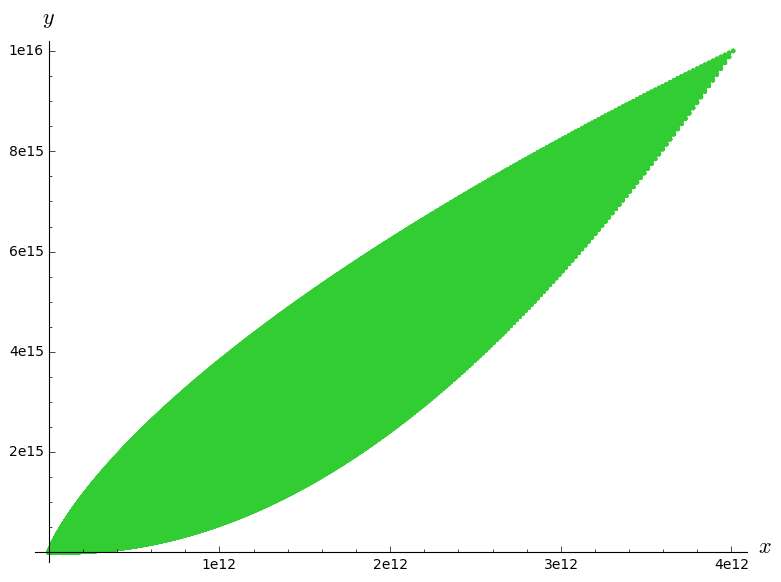
\includegraphics[width=1\textwidth]{plots/ch5_21_P6.png}
\vspace{-0.1cm}\caption{$\FFF(\PP_6)\leadsto 625.11$ s.}
\end{subfigure}
\hspace{0.8cm}
\begin{subfigure}{.38\linewidth}\centering
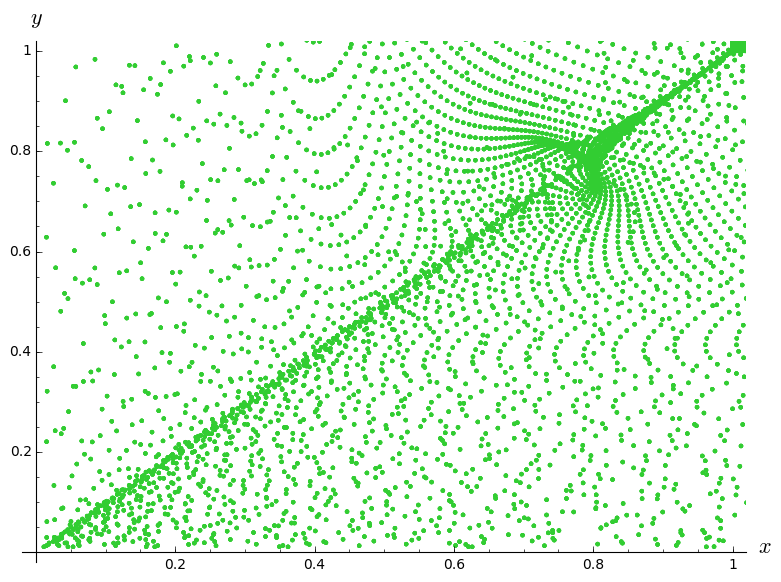
\includegraphics[width=1\textwidth]{plots/ch5_22_P6prime.png}
\vspace{-0.1cm}\caption{$\FFF(\PP_6)\leadsto 625.11$ s.}
\end{subfigure}
\end{figure}
\end{frame}

\begin{frame}
\frametitle{Randomly distributed points contained in a disc}
\begin{table}[ht!]
\begin{center}
\begin{tabular}{c || c | c | c}
& $g = \P\circ Q \circ H$ & $f=\HH\circ\GG\circ\FF$ & $\FFF$ \\ \hline \hline
${\mathbb D}_1$ & 131.97 s & 99.56 s & 32.02 s \\ \hline
${\mathbb D}_{100}$ & 131.62 s & 100.84 s & 32.36 s \\
\end{tabular}
\end{center}
\end{table}

\begin{figure}
\vspace{-0.25cm}
\begin{subfigure}{.32\linewidth}\centering
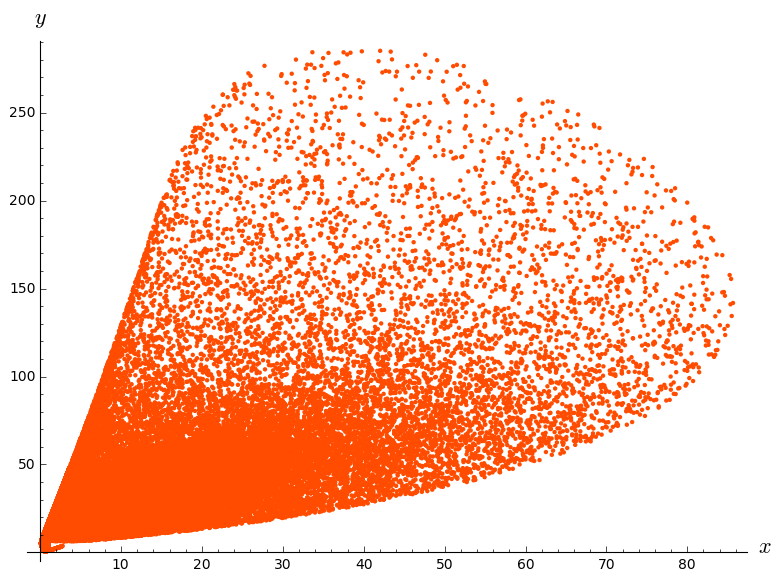
\includegraphics[width=1\textwidth]{plots/ch5_35_disc1.png}
\caption{$g({\mathbb D}_1)$.}
\end{subfigure}
\begin{subfigure}{.32\linewidth}\centering
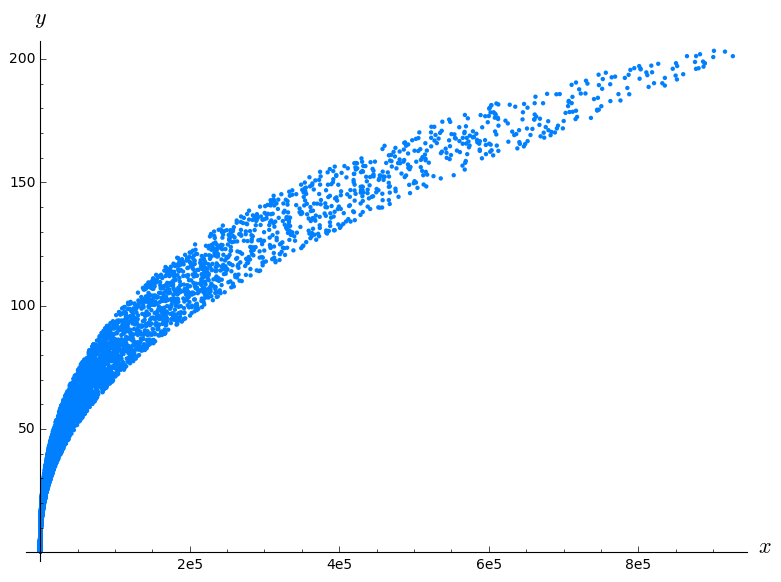
\includegraphics[width=1\textwidth]{plots/ch5_37_disc2.png}
\caption{$f({\mathbb D}_1)$.}
\end{subfigure}
\begin{subfigure}{.32\linewidth}\centering
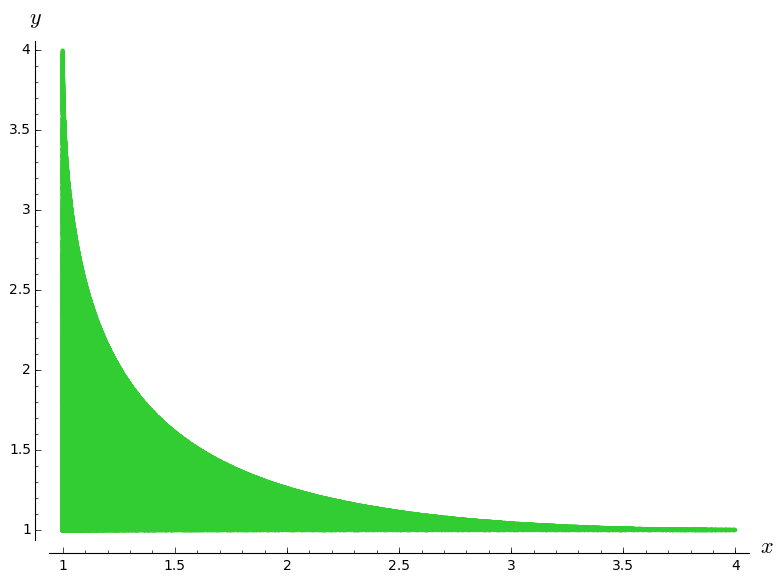
\includegraphics[width=1\textwidth]{plots/ch5_39_disc3.png}
\caption{$\FFF({\mathbb D}_1)$.}
\end{subfigure}
\end{figure}
\end{frame}

\begin{frame}
\frametitle{Using families of curves for $g$ and $f_2$}

\begin{figure}
\vspace{-0.2cm}
\begin{subfigure}{.28\linewidth}\centering
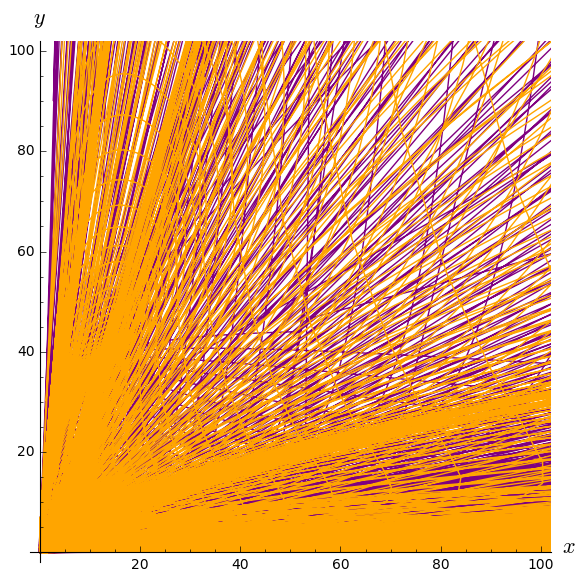
\includegraphics[width=1\textwidth]{plots/ch5_25_1curves3.png}
\vspace{-0.1cm}\caption{$g$ in $[0, 100]^2$.}
\end{subfigure} \hspace{0.4cm}
\begin{subfigure}{.28\linewidth}\centering
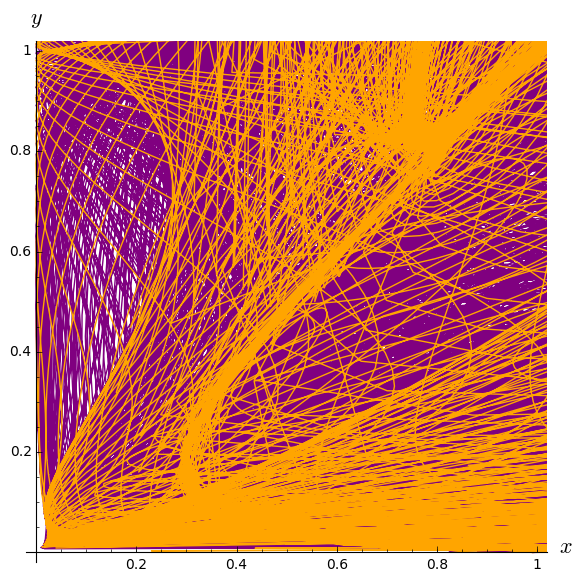
\includegraphics[width=1\textwidth]{plots/ch5_24_1curves2.png}
\vspace{-0.1cm}\caption{$g$ in $[0, 1]^2$.}
\end{subfigure} \hspace{0.4cm}
\begin{subfigure}{.28\linewidth}\centering
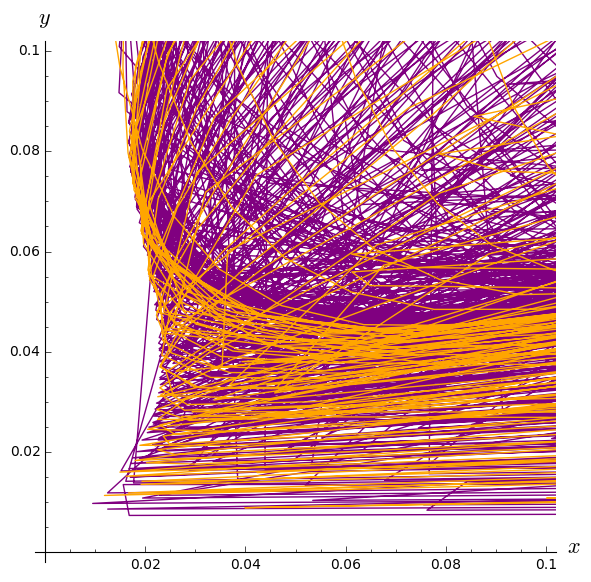
\includegraphics[width=1\textwidth]{plots/ch5_26_1curves4.png}
\vspace{-0.1cm}\caption{$g$ in $[0, 0.1]^2$.}
\end{subfigure}\\[1ex]
\vspace{0.1cm}
\begin{subfigure}{.28\linewidth}\centering
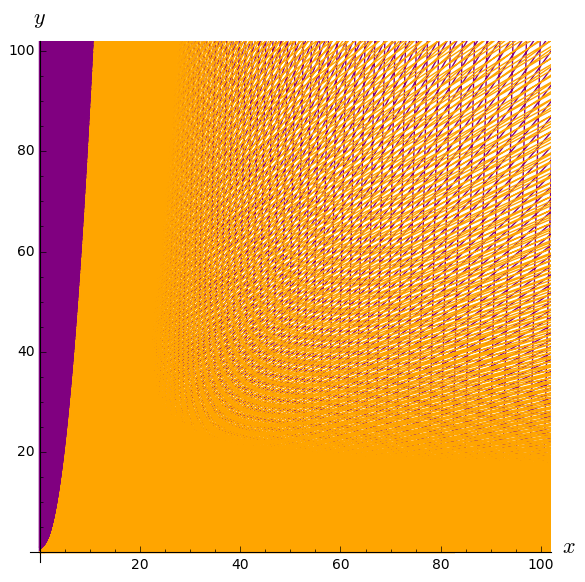
\includegraphics[width=1\textwidth]{plots/ch5_29_3curves3.png}
\vspace{-0.1cm}\caption{$f_2$ in $[0, 100]^2$.}
\end{subfigure} \hspace{0.4cm}
\begin{subfigure}{.28\linewidth}\centering
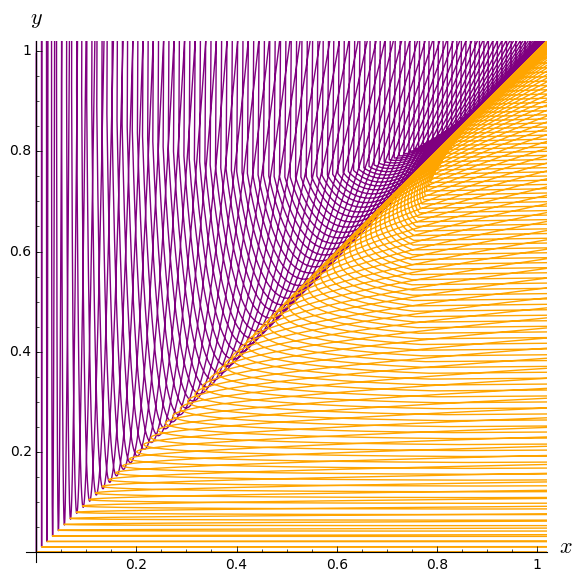
\includegraphics[width=1\textwidth]{plots/ch5_30_3curves4.png}
\vspace{-0.1cm}\caption{$f_2$ in $[0, 1]^2$.}
\end{subfigure} \hspace{0.4cm}
\begin{subfigure}{.28\linewidth}\centering
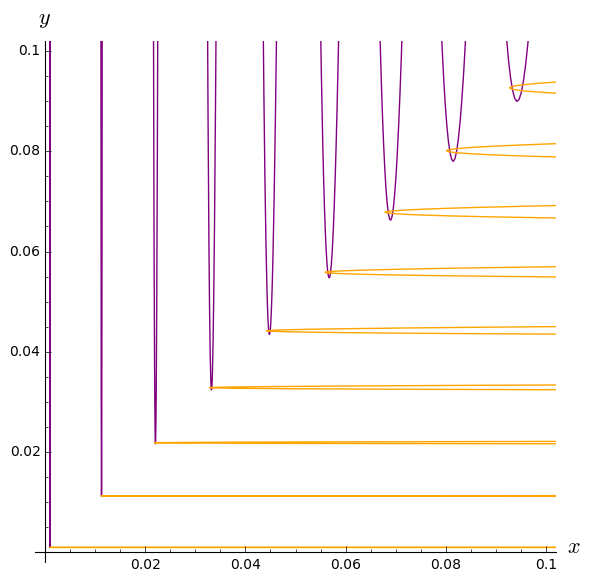
\includegraphics[width=1\textwidth]{plots/ch5_30_3curves5.png}
\vspace{-0.1cm}\caption{$f_2$ in $[0, 0.1]^2$.}
\end{subfigure}
\end{figure}
\end{frame}

\begin{frame}
\frametitle{Using families of curves for $\mathcal{N}_1$ and $\mathcal{N}_2$}

\begin{figure}
\vspace{-0.2cm}
\begin{subfigure}{.28\linewidth}\centering
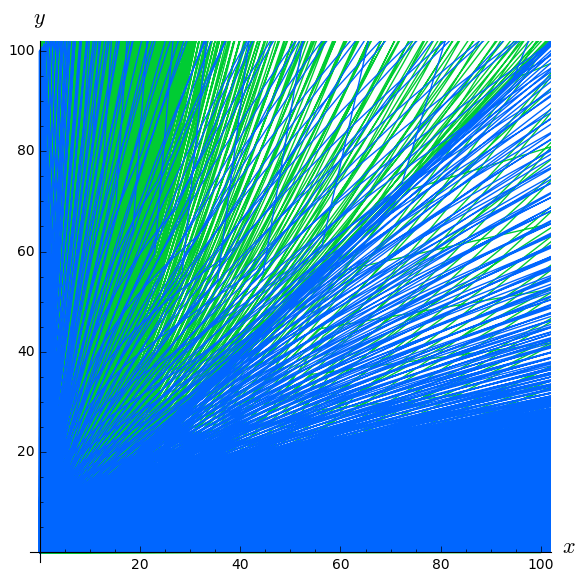
\includegraphics[width=1\textwidth]{plots/ch5_newCurves2.png}
\vspace{-0.1cm}\caption{$\mathcal{N}_1$ in $[0, 100]^2$.}
\end{subfigure} \hspace{0.4cm}
\begin{subfigure}{.28\linewidth}\centering
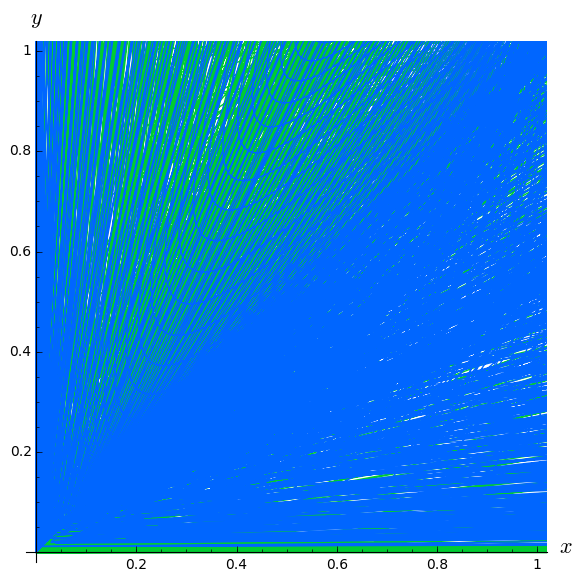
\includegraphics[width=1\textwidth]{plots/ch5_newCurves1.png}
\vspace{-0.1cm}\caption{$\mathcal{N}_1$ in $[0, 1]^2$.}
\end{subfigure} \hspace{0.4cm}
\begin{subfigure}{.28\linewidth}\centering
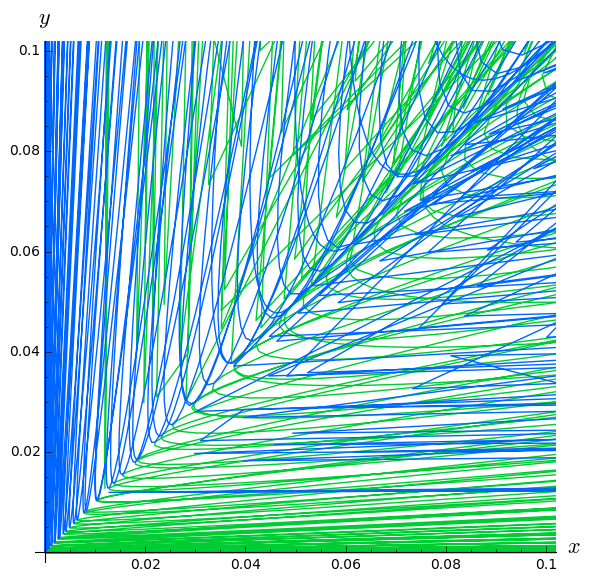
\includegraphics[width=1\textwidth]{plots/ch5_32_4curves2.png}
\vspace{-0.1cm}\caption{$\mathcal{N}_1$ in $[0, 0.1]^2$.}
\end{subfigure}\\[1ex]
\vspace{0.1cm}
\begin{subfigure}{.28\linewidth}\centering
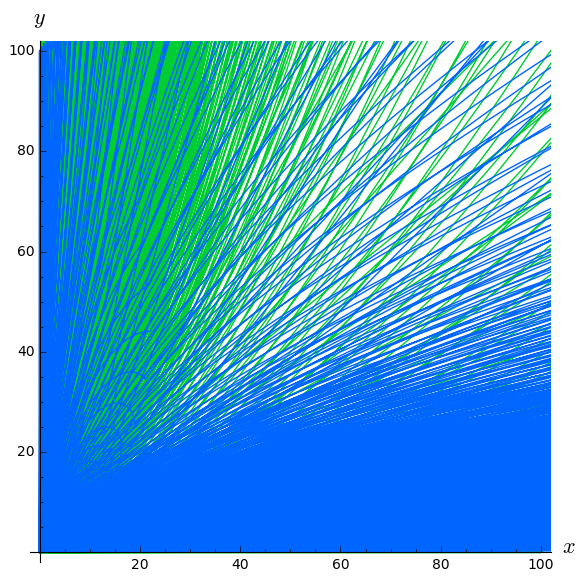
\includegraphics[width=1\textwidth]{plots/ch5_newCurves4.png}
\vspace{-0.1cm}\caption{$\mathcal{N}_2$ in $[0, 100]^2$.}
\end{subfigure} \hspace{0.4cm}
\begin{subfigure}{.28\linewidth}\centering
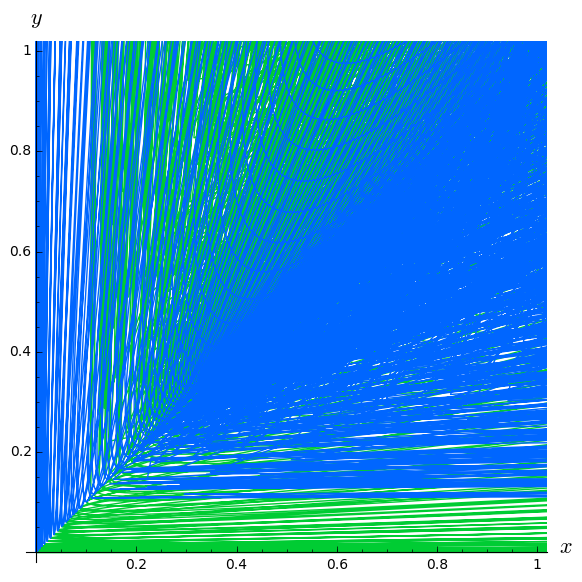
\includegraphics[width=1\textwidth]{plots/ch5_newCurves3.png}
\vspace{-0.1cm}\caption{$\mathcal{N}_2$ in $[0, 1]^2$.}
\end{subfigure} \hspace{0.4cm}
\begin{subfigure}{.28\linewidth}\centering
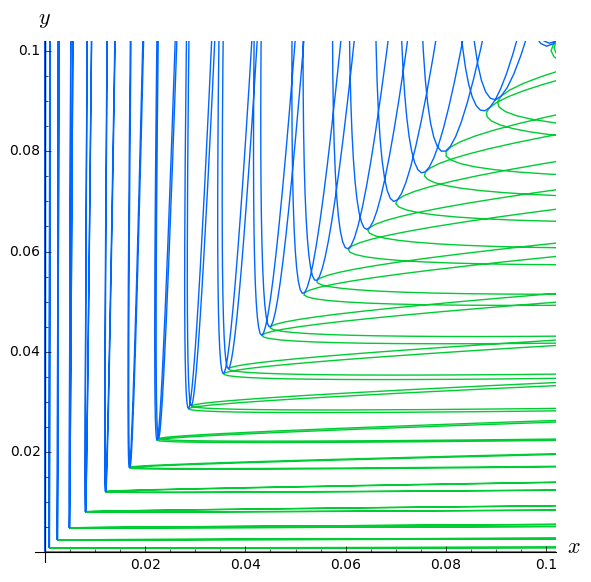
\includegraphics[width=1\textwidth]{plots/ch5_33_4curves3.png}
\vspace{-0.1cm}\caption{$\mathcal{N}_2$ in $[0, 0.1]^2$.}
\end{subfigure}
\end{figure}
\end{frame}

\section{ }
\subsection{ }
\begin{frame}
\frametitle{Some bibliography}\footnotesize{
\begin{thebibliography}{ABR}

\bibitem[BCR]{bcr} J. Bochnak, M. Coste, M.-F. Roy: G\'eom\'etrie alg\'ebrique r\'eelle. \em Ergeb. Math. \em {\bf 12}, Springer-Verlag, Berlin, Heidelberg, New York (1987).
\vspace{0.2cm}

\bibitem[FG]{fg} J.F. Fernando, J.M. Gamboa: Polynomial images of $\R^n$. {\em J. Pure Appl. Algebra}, {\bf179} (2003), 241--254.
\vspace{0.2cm}

\bibitem[FGU]{fgu} J.F. Fernando, J.M. Gamboa, C. Ueno: The open quadrant problem:
A topological proof.  A mathematical tribute to Professor Jos\'e Mar\'ia Montesinos. Departamento de Geometr\'ia y Topolog\'ia. Facultad de CC. Matem\'aticas UCM, (2016), 337--350.
\vspace{0.2cm}

\bibitem[FU1]{fu1} J.F. Fernando, C. Ueno: On the open quadrant as a polynomial image of $\R^2$ (revisited).
\vspace{0.2cm}

\bibitem[U]{u} C. Ueno: Im\'agenes polin\'omicas y regulares de espacios eucl\'\i deos. Ph.D. Thesis UCM, (2012).

\end{thebibliography}	}
\end{frame}

\beginbackup
\setbeamertemplate{footline}
{
\leavevmode%
\hbox{%
\begin{beamercolorbox}[wd=.4\paperwidth,ht=2.25ex,dp=1ex,center]{author in head/foot}%
\usebeamerfont{author in head/foot}\insertsection
\end{beamercolorbox}%
\begin{beamercolorbox}[wd=.35\paperwidth,ht=2.25ex,dp=1ex,center]{title in head/foot}%
\usebeamerfont{title in head/foot}\insertsubsection
\end{beamercolorbox}%
\begin{beamercolorbox}[wd=.25\paperwidth,ht=2.25ex,dp=1ex,right]{date in head/foot}%
\usebeamerfont{date in head/foot}\insertshortdate{}\hspace*{1em}
\insertframenumber{} \hspace*{3ex}
\end{beamercolorbox}}%
\vskip0pt%
}

%% TO DO: Meter animacion de las gammas y/o de las y^+, y^-
\begin{frame}
\frametitle{The first proof: $g:=\P\circ Q\circ H$}
$\star$ $\Qu \subset \P(\R^2) \leadsto$ Fix $v>0$ and proof that $\F\big(\{\G=v\}\big) \supset(0,+\infty)$: 
\vspace{0.4cm}

$\cdot $ \textbf{Step 1:}  Parametrization of the curve $\{\G-v=0\}$. Define $\gamma_v^+(\x, v):=\F(\x,y^+(\x,v))\text{ and }\gamma_v^-(\x, v):=\F(\x,y^-(\x,v)) \leadsto$ \vspace{-0.1cm}
$$
(0,+\infty)\overset{?}{\subset}\text{im}(\gamma_v^+)\cup\text{im}(\gamma_v^-).
$$ 
\vspace{-0.4cm}

$\cdot $ \textbf{Step 2:}  Main properties of $\gamma_v^+ \text{ and } \gamma_v^-$. Except for $\gamma_1^-(x)$, we have: \vspace{-0.1cm}
$$
\lim_{x\rightarrow \pm\infty}\gamma_v^+(x)=\lim_{x\rightarrow \pm\infty}\gamma_v^-(x)=0,\ \ \lim_{x\rightarrow 0}\gamma_v^+(x)=\lim_{x\rightarrow 0}\gamma_v^-(x) = +\infty.
$$ 
\vspace{-0.3cm}

$\cdot $ \textbf{Step 3:} When $v\geq 0.28^2$ we have $(0,+\infty)\subset\text{im}(\gamma_v^+)$.  
\vspace{0.4cm}

$\cdot $ \textbf{Step 4:} When $0<v<0.28^2$ we have $(0,+\infty)\subset\text{im}(\gamma_v^-)$.

\end{frame}


\begin{frame}
\frametitle{The short proof: The first lemma}

\begin{block}{Lemma 3.1}
\em Let $\mathscr{A}:=\set{xy\ge1}\ \cap\, \Qu$. Then the image of the map \vspace{-0.2cm}
$$
\FF:=(\FF_1,\FF_2):\R^2\to\R^2,(x,y)\mapsto((xy-1)^2+x^2,(xy-1)^2+y^2)
$$ \vspace{-0.7cm}

satisfies that $\mathscr{A}\subset\FF(\R^2)\subset\Qu$. \em 
\end{block}
\begin{figure}
\begin{tikzpicture}
\node[anchor=south west,inner sep=0] (img)at (0,0) {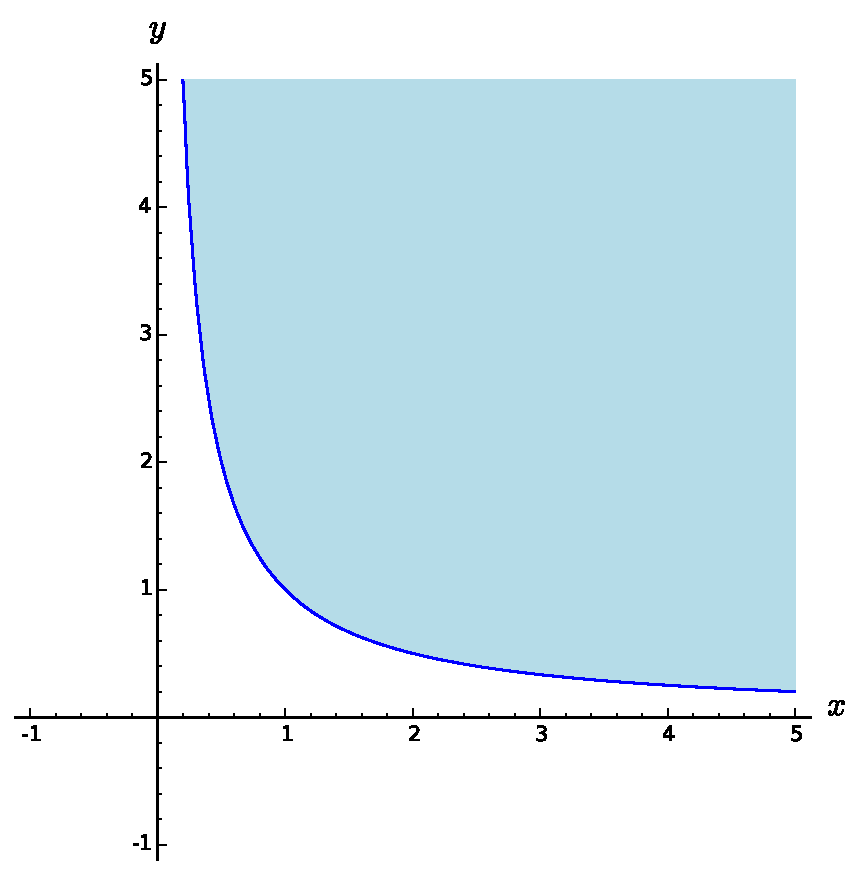
\includegraphics[width=0.4\textwidth]{plots/ch2_07_A.pdf}};
\path ($(img.north west)!0.6!(img.north east)$)|-coordinate(c1)($(img.south east)!0.7!(img.north east)$);% c1: lugar donde poner \mathscr{A}
\draw (c1) node {\large{$\mathscr{A}$}};
\end{tikzpicture}
\end{figure}

\end{frame}

\begin{frame}
\frametitle{The short proof: The second lemma}

\begin{block}{Lemma 3.2}
\em Let $\mathscr{B}:=\mathscr{A}\cup\set{y\ge x>0}$. Then, the map \vspace{-0.2cm}
$$
\GG:=(\GG_1,\GG_2):\R^2\to\R^2,(x,y)\mapsto (x,\ y(xy-2)^2+x(xy-1)^2)
$$ \vspace{-0.7cm}

satisfies that $\mathscr{B}\subset\GG(\mathscr{A})\subset\GG(\Qu)\subset\Qu$. \em 
\end{block}

\begin{columns}
\begin{column}{0.5\textwidth}

$$
y_x:=\text{min}\set{x,1/x},
$$

$$
\mathscr{B}_x:=[y_x,+\infty),
$$

$$
\mathscr{B}=\bigsqcup_{x>0}(\set{x}\times\mathscr{B}_x).
$$
\end{column}
\begin{column}{0.5\textwidth}
\begin{center}
\resizebox{5cm}{5cm}{%
\begin{tikzpicture}
\node[anchor=south west,inner sep=0] (img)at (0,0) {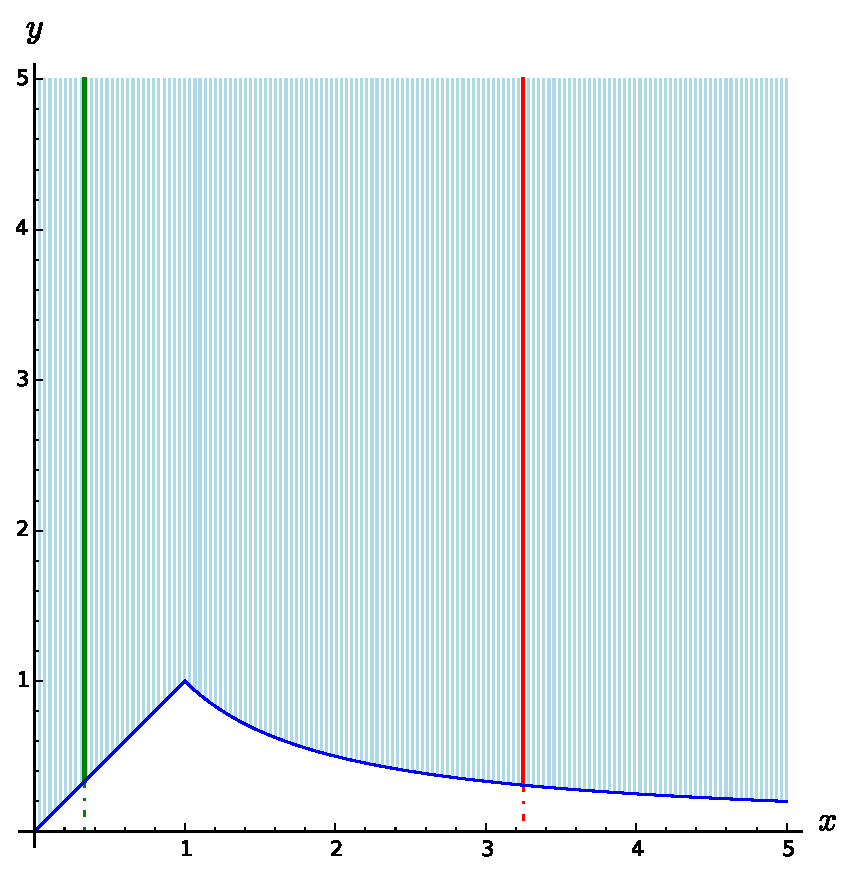
\includegraphics[width=1\textwidth]{plots/ch2_09_B_vert.pdf}};
\path ($(img.north west)!0.8!(img.north east)$)|-coordinate(c1)($(img.south east)!0.8!(img.north east)$); % Para \mathscr{B}
\path ($(img.north west)!0.1!(img.north east)$)|-coordinate(c2)($(img.south east)!0.89!(img.north east)$); % Para la flecha de x_0
\path ($(img.north west)!0.613!(img.north east)$)|-coordinate(c3)($(img.south east)!0.89!(img.north east)$); % Para la flecha de x_1
\path ($(img.north west)!0.1!(img.north east)$)|-coordinate(c4)($(img.south east)!0.105!(img.north east)$); % Para [
\path ($(img.north west)!0.613!(img.north east)$)|-coordinate(c5)($(img.south east)!0.101!(img.north east)$); % Para [
\path ($(img.north west)!0.1!(img.north east)$)|-coordinate(c6)($(img.south east)!0.01!(img.north east)$); % Para x_0
\path ($(img.north west)!0.613!(img.north east)$)|-coordinate(c7)($(img.south east)!0.01!(img.north east)$); % Para x_1
\path ($(img.north west)!0.26!(img.north east)$)|-coordinate(c8)($(img.south east)!0.55!(img.north east)$); % Para B_{x_0}
\path ($(img.north west)!0.77!(img.north east)$)|-coordinate(c9)($(img.south east)!0.35!(img.north east)$); % Para B_{x_1}
\draw (c1) node {\huge{$\mathscr{B}$}};
\draw (c2) node {\Large{\color[rgb]{0,0.392157,0}{$\uparrow$}}};
\draw (c3) node {\Large{\color[rgb]{1,0,0}{$\uparrow$}}};
\draw (c4) node {\large{\color[rgb]{0,0.392157,0}{\rotatebox[origin=c]{90}{[}}}};
\draw (c5) node {\large{\color[rgb]{1,0,0}{\rotatebox[origin=c]{90}{[}}}};
\draw (c6) node {\large{\color[rgb]{0,0.392157,0}{$x_0$}}};
\draw (c7) node {\large{\color[rgb]{1,0,0}{$x_1$}}};
\draw (c8) node {\large{\color[rgb]{0,0.392157,0}{$\set{x_0} \times \mathscr{B}_{x_0}$}}};
\draw (c9) node {\large{\color[rgb]{1,0,0}{$\set{x_1} \times \mathscr{B}_{x_1}$}}};
\end{tikzpicture}
}
\end{center}
\end{column}
\end{columns}

\end{frame}

\begin{frame}
\frametitle{The short proof: The third lemma}

\begin{block}{Lemma 3.3}
\em The polynomial map  \vspace{-0.2cm}
$$
\HH:=(\HH_1,\HH_2):\R^2\to\R^2,(x,y)\mapsto(x(xy-2)^2+\tfrac{1}{2}xy^2,\ y)
$$ \vspace{-0.7cm}

satisfies $\HH(\mathscr{B})=\HH(\Qu)=\Qu$. \em 
\end{block}
\begin{columns}
\begin{column}{0.5\textwidth}

$$\mathscr{C}_y:= 
\left\{
\begin{array}{ll}
\!\!\!(0,+\infty)&\!\!\!\text{if } y \ge 1,\\
\!\!\!(0,y]\cup[1/y,+\infty) & \!\!\!\text {if } 0<y<1.
\end{array}
\right.
$$

$$
\mathscr{B}=\bigsqcup_{y>0}(\mathscr{C}_y\times\set{y}).
$$

\end{column}
\begin{column}{0.5\textwidth}


\begin{center}
\resizebox{5cm}{5cm}{%
\begin{tikzpicture}
\node[anchor=south west,inner sep=0] (img)at (0,0) {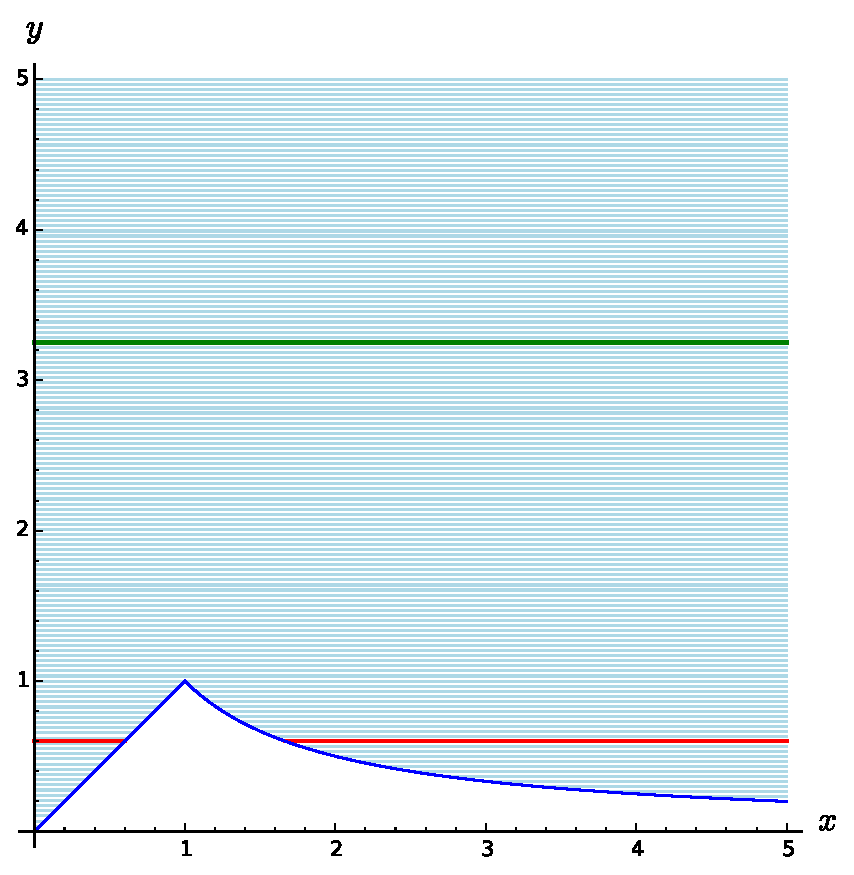
\includegraphics[width=1\textwidth]{plots/ch2_10_B_hor.pdf}};
\path ($(img.north west)!0.6!(img.north east)$)|-coordinate(c1)($(img.south east)!0.7!(img.north east)$);% c1: lugar donde poner \mathscr{B}
\path ($(img.north west)!0.8!(img.north east)$)|-coordinate(c1)($(img.south east)!0.8!(img.north east)$); % Para \mathscr{B}
\path ($(img.north west)!0.9!(img.north east)$)|-coordinate(c2)($(img.south east)!0.604!(img.north east)$); % Para la flecha de y_0
\path ($(img.north west)!0.9!(img.north east)$)|-coordinate(c3)($(img.south east)!0.1492!(img.north east)$); % Para la flecha de y_1
\path ($(img.north west)!0.045!(img.north east)$)|-coordinate(c4)($(img.south east)!0.61!(img.north east)$); % Para (
\path ($(img.north west)!0.045!(img.north east)$)|-coordinate(c5)($(img.south east)!0.154!(img.north east)$); % Para (
\path ($(img.north west)!0.146!(img.north east)$)|-coordinate(c10)($(img.south east)!0.154!(img.north east)$); % Para ]
\path ($(img.north west)!0.335!(img.north east)$)|-coordinate(c11)($(img.south east)!0.154!(img.north east)$); % Para [
\path ($(img.north west)!0.008!(img.north east)$)|-coordinate(c6)($(img.south east)!0.61!(img.north east)$); % Para y_0
\path ($(img.north west)!0.008!(img.north east)$)|-coordinate(c7)($(img.south east)!0.154!(img.north east)$); % Para y_1
\path ($(img.north west)!0.25!(img.north east)$)|-coordinate(c8)($(img.south east)!0.66!(img.north east)$); % Para B_{y_0}
\path ($(img.north west)!0.65!(img.north east)$)|-coordinate(c9)($(img.south east)!0.2!(img.north east)$); % Para B_{y_1}
\draw (c1) node {\huge{$\mathscr{B}$}};
\draw (c2) node {\Large{\color[rgb]{0,0.392157,0}{$\rightarrow$}}};
\draw (c3) node {\Large{\color[rgb]{1,0,0}{$\rightarrow$}}};
\draw (c4) node {\large{\color[rgb]{0,0.392157,0}{(}}};
\draw (c5) node {\large{\color[rgb]{1,0,0}{(}}};
\draw (c10) node {\large{\color[rgb]{1,0,0}{]}}};
\draw (c11) node {\large{\color[rgb]{1,0,0}{[}}};
\draw (c6) node {\large{\color[rgb]{0,0.392157,0}{$y_0$}}};
\draw (c7) node {\large{\color[rgb]{1,0,0}{$y_1$}}};
\draw (c8) node {\large{\color[rgb]{0,0.392157,0}{$\mathscr{C}_{y_0} \times \set{y_0}$}}};
\draw (c9) node {\large{\color[rgb]{1,0,0}{$\mathscr{C}_{y_1} \times \set{y_1}$}}};
\end{tikzpicture}
}
\end{center}
\end{column}
\end{columns}

\end{frame}

\begin{frame}
\frametitle{The short proof}
\begin{block}{Lemma 3.1}
The polynomial map $\FF$ verifies that $\mathscr{A}\subset\FF(\R^2)\subset\Qu$.
\end{block}
\begin{block}{Lemma 3.2}
The polynomial map $\GG$ verifies that $\mathscr{B}\subset\GG(\mathscr{A})\subset\GG(\Qu)\subset\Qu$.
\end{block}
\begin{block}{Lemma 3.3}
The polynomial map $\HH$ verifies that $\HH(\mathscr{B})=\HH(\Qu)=\Qu$.
\end{block}

$$
\!\!\!\Qu\overset{3.3}{=}\HH(\mathscr{B})\!\overset{3.2}{\subset}\!(\HH\circ\GG)(\mathscr{A})
\!\overset{3.1}{\subset}\!(\HH\circ\GG\circ\FF)(\R^2) \!\overset{3.1}{\subset}\!(\HH\circ\GG)(\Qu) \!\overset{3.2}{\subset}\!\HH(\Qu)\overset{3.3}{=}\Qu.
$$
\end{frame}

\begin{frame}
\frametitle{The topological proof: $\FFF=f_2\circ f_1$} 
$\cdot$ \textbf{Step 1:} Factor $\FFF=f_2\circ f_1$, with: \vspace{-0.2cm}
\begin{align*}
&f_1(\x,\y):=\big(\x^2,\,\y^2\big) \leadsto f_1\big(\R^2\big)=\overline{\Qu}:=\set{x\ge 0,y\ge 0},\\
&f_2(\x,\y):=\big((\x\y^2+\x^2\y-\y-1)^2+\x^3\y^2,\,(\x^3\y+\x\y-\x-1)^2+\x^3\y^2\big).
\end{align*}\vspace{-0.6cm} 

$\cdot$ \textbf{Step 2:} Factor $f_2=h\circ g$, where $g:\overline{\Qu}\to\R^3,\ h:\R^3\to\R^2$ and: \vspace{-0.2cm}
\begin{align*}
g(\x,\y)&:=\big(\x\y^2+\x^2\y-\y-1,\,\x^{3/2}\y,\,\x^3\y+\x\y-\x-1\big),\\
h(\x,\y,\z)&:=\big(\x^2+\y^2,\,\y^2+\z^2\big).
\end{align*}\vspace{-0.6cm} 

$\cdot$ \textbf{Step 3:} Let $\Ss:=g\big(\overline{\Qu}\big)$. Then:  \vspace{-0.2cm}
$$
\forall\, \,  (A^2,B^2)\in\Qu:\ h^{-1}\big(\set[\big]{(A^2,B^2)}\big)\ \bigcap\ \Ss\ne\varnothing.
$$\vspace{-0.6cm}  

$\cdot$ \textbf{Step 4:} For fixed values $B\ge A>0$: $\partial\D_1\cap\Ss \ne \varnothing \ne \partial\D_2\cap\Ss$.

\end{frame}

\begin{frame}
\frametitle{The topological proof: \textbf{Step 4}}

\begin{columns}
\begin{column}{0.5\textwidth}
\begin{center}The boundary map $\partial\tilde{\phi}_M:\partial\tilde{\overline{\Rr}}_M\rightarrow\R^3$ meets transversally once $\D_1$.
\end{center}\begin{figure}[!ht]
\begin{center}
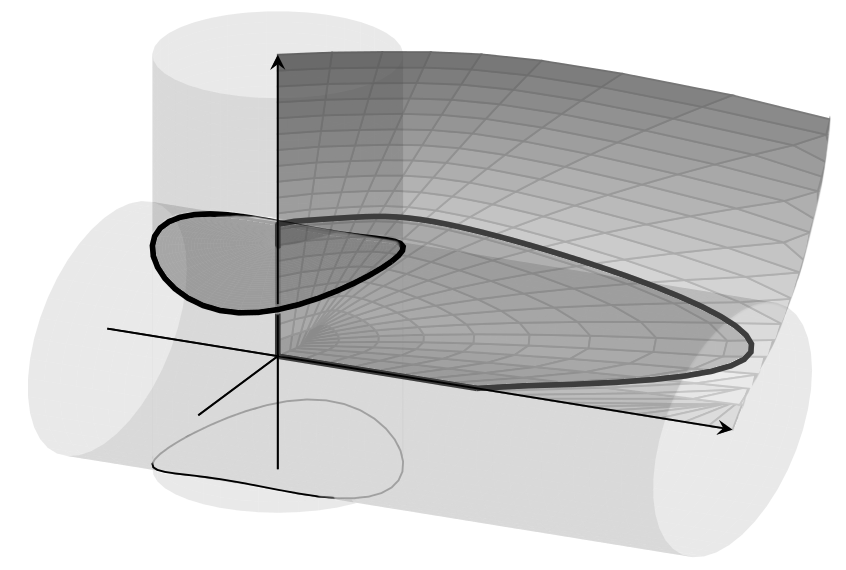
\includegraphics[height=4cm]{plots/ch3_02_B2.png}
\end{center}
\end{figure}
\end{column}
\begin{column}{0.5\textwidth}
\begin{center}The boundary map $\partial\tilde{\phi}_M:\partial\tilde{\overline{\Rr}}_M\rightarrow\R^3$ meets transversally once $\D_2$.
\end{center}\begin{figure}[!ht]
\begin{center}
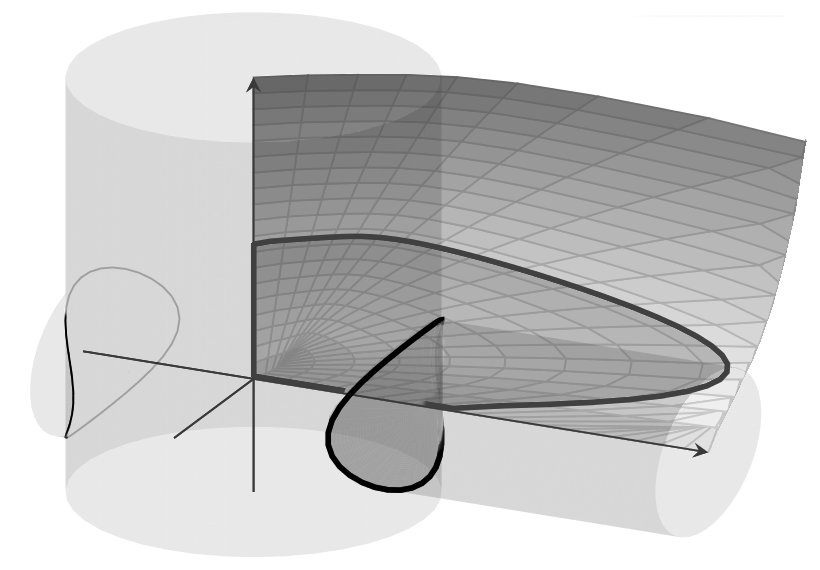
\includegraphics[height=4cm]{plots/ch3_01_A2.png}
\end{center}
\end{figure}
\end{column}
\end{columns}

\end{frame}
\backupend

\end{document}